\chapter{Логические, продукционные и функциональные модели решения задач в ostis-системах}
\chapauthortoc{Ивашенко В.~П.\\Шункевич Д.~В.\\Василевская А.~П.\\Орлов М.~К.}
\label{chapter_logic_productions}

\begin{SCn}
	\begin{scnrelfromlist}{автор}
		\scnitem{Ивашенко В.~П.}
		\scnitem{Шункевич Д.~В.}
		\scnitem{Василевская А.~П.}
		\scnitem{Орлов М.~К.}
	\end{scnrelfromlist}
\end{SCn}

\bigskip

\abstract{Логические модели решения задач являются основой обработки знаний в \textit{интеллектуальных системах}. В данной главе рассматривается интеграция различных \textit{моделей решения задач}, в том числе принципы \textit{логического вывода}, для решения задач на основе общей формальной модели.}

\bigskip

\begin{SCn}
\begin{scnrelfromlist}{библиографическая ссылка}
	\scnitem{\scncite{Lawan2019}}
	\scnitem{\scncite{Golenkov1996_2}}
	\scnitem{\scncite{Averin2004}}
	\scnitem{\scncite{Golenkov2004}}
	\scnitem{\scncite{Sethy2021}}
	\scnitem{\scncite{Norton2019}}
	\scnitem{\scncite{Yuxuan2022}}
	\scnitem{\scncite{Safawi2015}}
	\scnitem{\scncite{Gungov2018}}
	\scnitem{\scncite{Geramian2017}}
	\scnitem{\scncite{Son2017}}
	\scnitem{\scncite{Uehara2017}}
	\scnitem{\scncite{Lupea2002}}
	\scnitem{\scncite{Weydert2022}}
	\scnitem{\scncite{Chen2021}}
	\scnitem{\scncite{Rybakov2020}}
	\scnitem{\scncite{Orlov2022b}}
	\scnitem{\scncite{Gavrilova2001}}
	\scnitem{\scncite{AIHandbookMM}}
	\scnitem{\scncite{Brownston1985}}
	\scnitem{\scncite{CLIPS}}
	\scnitem{\scncite{Forgy1982}}
	\scnitem{\scncite{Vladimirov2010}}
\end{scnrelfromlist}
\end{SCn}

\bigskip

\begin{SCn}
\begin{scnrelfromlist}{подраздел}
	\scnitem{\ref{logic_lang_os}~\nameref{logic_lang_os}}
	\scnitem{\ref{sec_logic_productions}~\nameref{sec_logic_productions}}
\end{scnrelfromlist}
\end{SCn}

\section{Операционная семантика логических языков, используемых ostis-системами}
\label{logic_lang_os}

\begin{SCn}
	\begin{scnrelfromlist}{ключевой знак}
		\scnitem{Язык SCL}
		\scnitem{Абстрактная scl-машина}
	\end{scnrelfromlist}
\end{SCn}

\begin{SCn}
	\begin{scnrelfromlist}{ключевое понятие}
		\scnitem{логический вывод}
	\end{scnrelfromlist}
\end{SCn}

\bigskip

\begin{SCn}
	\begin{scnrelfromlist}{ключевое знание}
		\scnitem{Формализация правила вывода Modus ponens}
		\scnitem{Формализация правила резолюции}
		\scnitem{Спецификация агента прямого логического вывода}
	\end{scnrelfromlist}
\end{SCn}

\bigskip

Логика решает задачи доказательства высказываний, аргументации того или иного высказывания, задачу генерации и опровержения гипотез. Некоторые гипотезы могут быть опровергнуты, однако извлекая причины того, почему гипотеза опровергнута, можно изменить посылку гипотезы так, чтобы создать новую гипотезу, которая впоследствии может стать теоремой.

Современная логика изучает \textit{формальные языки}, служащие для выражения логических рассуждений. \textit{логический язык} — \textit{формальный язык}, предназначенный для воспроизведения логических форм контекстов \textit{естественного языка}, а также выражения логических законов и способов правильных рассуждений в логических теориях, строящихся в данном языке. Логика не изучает то, как были получены знания, она позволяет представлять знания, а также из существующих знаний вывести новые (то есть из имеющихся формул логики вывести новые формулы этой же логики), установить правильность рассуждений.

На данный момент реализовано много систем \textit{логического вывода}, использующих известные правила прямого заключения и резолюции в различных видах логик, однако остаются актуальными проблема совместимости вышеописанных систем и проблема коллективного решения задач с использованием различных моделей решения задач.

Каждая модель решения задач задается языком, обеспечивающим представление в памяти кибернетической системы некоторого класса методов решения задач, и интерпретатором указанных методов, определяющим операционную семантику указанного языка. Следует рассмотреть языки, которыми может задаваться логическая модель решения задач. Такими языками являются \textit{Rule Interchange Format} (RIF), Semantic Web Rule Language (SWRL), \textit{SHACL Rules} и \textit{Notation3 Rules}, которые используются в \textit{Semantic Web} (см. \scncite{Lawan2019}). На \textit{\nameref{fig:swrl_example}} представлен пример правил на \textit{Языке SWRL}.

\begin{figure}[H]
	\caption{Рисунок. Запись правил на языке SWRL}
	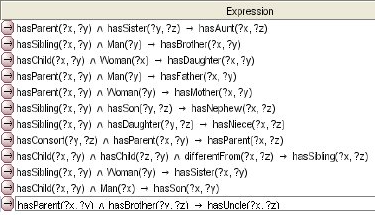
\includegraphics[scale=0.8]{author/part3/figures/swrl_example.png}
	\label{fig:swrl_example}
\end{figure}

Описанные языки не предусматривают возможность представления формул в различных видах логик, поэтому при помощи них невозможно решить описанные проблемы. Языки правил специально построены для вывода следствий. Синтаксис и семантика языков онтологий и языков правил довольно сильно отличаются, поэтому возникает вопрос, как их совмещать. 

\textbf{\textit{Пролог}} --- язык и система логического программирования. \textit{база знаний} системы \textit{Пролог} содержит информацию в виде предикатов. В логическом программировании, реализованном в \textit{Прологе}, используется только одно \textit{правило вывода} --- правило резолюции. Задача пролог-программы заключается в том, чтобы доказать, является ли заданное целевое высказывание следствием из имеющихся формул и, если является, то каким образом был получен такой вывод. Когда пользователь задает вопрос системе Пролог, система ищет соответствующие предикаты в базе знаний и, если они найдены, сравнивать их с заданными условиями. Система Пролог хорошо справляется с нетрудными задачами, однако ограничен лишь одним принципом логического вывода и не позволяет учитывать сложноструктурированные знания в различных видах логик.

Для решения указанных проблем предлагается \textit{логический язык} на основе \textit{SC-кода} и абстрактная машина логического вывода на основе предложенного языка. 

\textit{Технология OSTIS} позволяет интегрировать любые принципы логического вывода для решения задач в интеллектуальных системах на основе общей формальной модели. Для того, чтобы использовать какую-либо новую или существующую модель, необходимо привести ее к предлагаемому формализму, что позволит интегрировать и синхронизировать ее с уже имеющимися в соответствующей \textit{библиотеке многократно используемых компонентов ostis-систем}. Формализм \textit{SC-кода} позволяет описывать широкий спектр понятий и отношений между ними, что делает его подходящим вариантом для реализации логического вывода в интеллектуальных компьютерных системах нового поколения. Кроме того, целесообразно воспользоваться принципом наследования, лежащим в основе иерархической структуризации баз знаний ostis-систем. Исходя из этого предлагается следующая иерархия интегрированных предметных областей:

\begin{SCn}
	\scnheader{Предметная область логических формул, высказываний и формальных теорий}
	\begin{scnrelfromlist}{дочерняя предметная область}
		\scnitem{Предметная область логических языков}
		\scnitem{Предметная область логического вывода}
	\end{scnrelfromlist}
	
	\scnheader{Предметная область логических языков}
	\scnrelfrom{дочерняя предметная область}{Предметная область языка логики высказываний}
	\begin{scnindent}
		\scnrelfrom{дочерняя предметная область}{Предметная область языка логики предикатов}
	\end{scnindent}
	
	\scnheader{Предметная область логических моделей решения задач}
	\begin{scnreltolist}{дочерняя предметная область}
		\scnitem{Предметная область логических языков}
		\scnitem{Предметная область логического вывода}
	\end{scnreltolist}
\end{SCn}

Наследование предметных областей позволяет использовать описанные логики и их компоненты при описании любых логик. Базовые понятия позволяют разработчикам интеллектуальной системы добавлять новые логики. Для реализации конкретной логической модели решения задач необходимо создать предметную область, которая будет дочерней по отношению к \textit{Предметной области логических моделей решения задач} и предметной области некоторого \textit{логического языка}, например, языка логики высказываний, языка логики предикатов, языка нечеткой логики и других.

\textit{Предметная область логических формул, высказываний и формальных теорий} задает денотационную семантику логических формул, высказываний и формальных теорий и содержит формальную спецификацию понятий, необходимых для формирования логических формул и высказываний любых логик, в том числе традиционных, нечетких, правдоподбных, темпоральных, логик умолчания и любых других. Логические формулы и высказывания интерпретируется с помощью понятий, описанных в \textit{Предметной области логических моделей решения задач}, включающую модель и реализацию абстрактных агентов, необходимых для решения логических задач. Эта предметная область включает в себя спецификацию таких понятий, как логический вывод, правила вывода, равносильные преобразования и аксиомные схемы.

% Источник этого текста и используемых в нем ссылок здесь https://libeldoc.bsuir.by/bitstream/123456789/30629/1/Golenkov_Grapho.pdf
\textit{\textbf{Язык SCL}} — подъязык \textit{SC-кода} для записи логических утверждений (см. \scncite{Golenkov1996_2}), он подробно рассматривается в  \textit{Главе \ref{chapter_logic}~\nameref{chapter_logic}}. Над высказываниями \textit{Языка SCL} можно проводить \textit{логический вывод}.

Выводом в формальной системе называется любая последовательность формул такая, что любая формула либо аксиома этой формальной системы, либо непосредственное следствие каких-либо предыдущих формул по одному из правил вывода. Идея выводимости центральна в логике: в любой формальной аксиоматической теории теорема --- это формула, которая выводится из аксиом. Правильность умозаключений вводится и проверяется совершенно формально, без какой-либо связи с истинностью входящих в него посылок, то есть исключительно с точки зрения структуры рассуждения. С практической точки зрения самое важное свойство такой формальной правильности рассуждений заключается в следующем: если нам удалось доказать, пользуясь методами формальной логики, правильность рассуждения, и нам известно из опыта, что все используемые посылки истинны, то мы можем быть уверены в истинности заключения (см. \scncite{Averin2004}). Истинность используемых посылок задается состоянием базы знаний.

Различные логические подходы позволяют проектировать \textit{решатели задач} для \textit{интеллектуальных систем} в разных предметных областях, учитывая их специфику. \textit{решатель задач} каждой конкретной системы во многом зависит от назначения данной системы, множества решаемых задач, предметной области и других факторов (см. \textit{Главу \ref{chapter_situation_management}~\nameref{chapter_situation_management}}). Некоторые операции, необходимые в одной предметной области будут избыточными в другой. Например, в системе, решающей задачи по геометрии, химии и другим естественным наукам обоснованным будет использование дедуктивных методов вывода, поскольку решение задач в таких предметных областях основывается только на достоверных правилах. В системах же медицинской диагностики, к примеру, постоянно возникает ситуация, когда диагноз может быть поставлен только с некоторой долей уверенности и абсолютно достоверным ответ на поставленный вопрос быть не может. В связи с этим возникает необходимость использования различных \textit{решателей задач} в различных системах, при этом их состав и возможности в конкретной системе определяется не только непосредственно разработчиком, а требует консультаций с экспертами в данной предметной области. Тем не менее основой для всех видов логик является классическая логика и наиболее общие ее методы распространяются на другие логики с некоторыми модификациями, уточнениями и ограничениями (см. \scncite{Golenkov2004}).

Приведем краткую классификацию существующих логических методов решения задач:
\begin{textitemize}
	\item{\textbf{Классический дедуктивный вывод.} Классический дедуктивный вывод является наиболее популярным при построении автоматических решателей задач, так как всегда дает достоверный результат. Дедуктивный вывод включает в себя прямой и обратный и логический вывод (принцип резолюции, процедуру Эрбрана и так далее) (см. \scncite{Averin2004}), все виды силлогизмов (см. \scncite{Sethy2021}) и так далее. Основной проблемой дедуктивного вывода является невозможность его использования в ряде случаев, когда отсутствуют достоверные знания.}
	\item{\textbf{Индуктивный вывод.} Индуктивный вывод предоставляет возможность в процессе решения использовать различные предположения, что делает его удобным для использования в слабоформализованных и трудноформализуемых предметных областях, например при построении систем медицинской диагностики. Подробно принципы индуктивного вывода рассмотрены в работах \scncite{Norton2019}, \scncite{Yuxuan2022}.}
	\item{\textbf{Абдуктивный вывод.} Под абдуктивным выводом в искусственном интеллекте, как правило, понимается вывод наилучшего абдуктивного объяснения, то есть объяснения некоторого события, ставшего неожиданным для системы. Причем наилучшим считается такое объяснение, которое удовлетворяет специальным критериям, определяемым в зависимости от решаемой задачи и используемой	формализации. Абдуктивный вывод подробно рассматривается в работах \scncite{Safawi2015}, \scncite{Gungov2018}.}
	\item{\textbf{Нечеткая логика.} Теория нечетких множеств и, соответственно, нечетких логик, также применяется в системах, связанных с трудноформализуемыми предметными областями (см. \scncite{Geramian2017}, \scncite{Son2017}). Здесь импликативные высказывания могут рассматриваться как "если истинна посылка"{}, то с некоторой вероятностью (часто или редко) истинно заключение, в отличие от классической логики, где зачастую используются статические предметные области и выражение "часто или редко"{} не применимо (корректно использовать только наречие "всегда"{}). Подробнее теория нечетких логик рассматривается в работе \scncite{Uehara2017}.}
	\item{\textbf{Логика умолчаний.} Логика умолчаний применяется, в том числе, для того, чтобы оптимизировать процесс рассуждений,	дополняя процесс достоверного вывода вероятностными  предположениями в тех случаях, когда вероятность ошибки крайне мала. Подробнее логика умолчаний рассмотрена в статьях \scncite{Lupea2002}, \scncite{Weydert2022}.}
	\item{\textbf{Темпоральная логика.} Применение темпоральной логики является очень актуальным для нестатичных предметных областей, в которых истинность того или иного утверждения меняется со временем, что существенно влияет на ход решения какой-либо задачи (см. \scncite{Chen2021}, \scncite{Rybakov2020}). Следует отметить, что используемый в данной работе язык представления знаний предоставляет все необходимые возможности для описания таких динамических предметных областей.}
\end{textitemize}

База знаний интеллектуальной системы включает в себя как модель фактографических знаний о предметной области, для которой предназначена система, так и модель знаний, включающая в себя логические формулы об этой предметной области (аксиомы, теоремы и правила вывода).

\textit{\textbf{Абстрактная scl-машина}} является машиной логического вывода и относится к классу абстрактных sc-машин (см. \scncite{Golenkov1996_2}). Внутренним языком \textit{scl-машины} является указанный выше графовый логический \textit{Язык SCL}, ее операции соответствуют правилам \textit{логического вывода}. Семейство специализированных абстрактных графодинамических машин обработки знаний является формальным уточнением операционной семантики указанных выше специализированных графовых языков представления знаний, каждому из которых соответствует одна или несколько абстрактных машин. Эти абстрактные машины соответствуют различным моделям решения задач, различным логикам, различным моделям правдоподобных рассуждений. 
Агент из семейства агентов логического вывода может представлять собой какое-либо правило вывода, которое можно применять для решения логической задачи. Кроме того, необходимы агенты для выполнения равносильных преобразований логической формулы (например, записать формулу эквиваленции как конъюнкцию двух дизъюнкций) и другие агенты, помогающие применять правила вывода на множестве формул языка логики (см. \scncite{Orlov2022b}).

% Показать разные scl-машины в разных логиках. Дедуктивный вывод это база
\begin{SCn}
\scnheader{Абстрактная scl-машина}
\begin{scnrelfromset}{декомпозиция абстрактного sc-агента}
	\scnitem{Абстрактный sc-агент применения правила вывода}
	\scnitem{Абстрактный sc-агент эквивалентных преобразований логической формулы}
	\scnitem{Абстрактный sc-агент прямого логического вывода}
	\scnitem{Абстрактный sc-агент обратного логического вывода}
\end{scnrelfromset}
\scnhaselement{Реализации интерпретатора логических моделей решения задач}
\begin{scnindent}
	\scnidtf{Реализация scl-машины}
	\scntext{адрес компонента}{https://github.com/ostis-ai/scl-machine}
\end{scnindent}
\end{SCn}

Задачей \textit{Абстрактного sc-агента применения правила вывода} является применение заданного правила вывода с заданными логическими формулами. Данный sc-агент активируется при появлении в sc-памяти инициированного действия, принадлежащего классу \textit{действие применение правила вывода}. После проверки sc-агентом условия инициирования выполняется процесс применения правила вывода, который заключается в  проверке, существует ли в sc-памяти структуры, соответствующие условию применения данного правила и генерации sc-конструкций в соответствии с применяемым правилом. В ходе работы агента автоматически выполняется процедура унификации: переменные соответствуют константам, константы соответствуют самим себе. Агент применения правила вывода зачастую используется в процессе работы агентов прямого логического вывода, обратного логического вывода и других агентов. Примером правила вывода может быть правило прямого заключения (Modus ponens), представленное на рисунке \textit{\nameref{fig:modus_ponens_formalization}}.

\begin{figure}[H]
	\caption{SCg-текст. Формализация правила вывода Modus ponens}
	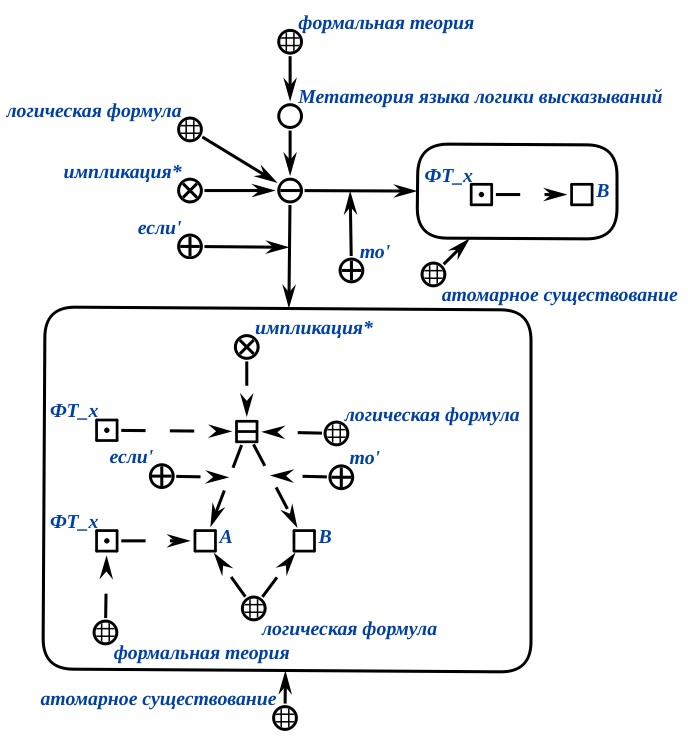
\includegraphics[scale=0.6]{author/part3/figures/Modus_ponens.png}
	\label{fig:modus_ponens_formalization}
\end{figure}

Можно привести еще целый ряд высказываний, которые описывают общие свойства всевозможных формальных теорий, каждая из которых описывает ту или иную предметную область. Свойства всевозможных формальных теорий описываются в рамках специальной метатеории для которой совокупность всевозможных формальных теорий является описываемой предметной областью.

Задачей \textit{Абстрактного sc-агента эквивалентных преобразований логической формулы} является применение некоторых правил, которые приводят логическую формулу в определенный вид. Данный sc-агент активируется при появлении в sc-памяти инициированного действия, принадлежащего классу \textit{действие эквиалентное преобразование логической формулы}. После проверки sc-агентом условия инициирования выполняется процесс преобразования формулы из одной формы в другую, при этом никакие новые знания в sc-памяти с точки зрения исследуемой предметной области не генерируются. Ответом данного агента является множество формул, эквивалентных по смыслу, но различных по форме представления. Такими формами могут быть, например, конъюнктивная нормальная форма или дизъюнктивная нормальная форма. Агент эквивалентных преобразований зачастую вызывается в процессе работы агента применения правила вывода, так как логические формулы не всегда находятся в той форме, которая доступна для применения того или иного правила вывода, однако может быть приведена к нужной форме.

Задачей \textit{Абстрактного sc-агента прямого логического вывода} является генерации новых знаний на основе некоторых логических утверждений. Данный sc-агент активируется при появлении в sc-памяти инициированного действия, принадлежащего классу \textit{действие прямого логического вывода}. После проверки sc-агентом условия инициирования выполняется процесс прямого логического вывода, который состоит из циклических операций применения правил вывода, генерации новых знаний в sc-памяти и проверки некоторого условия, например, появление в памяти sc-элементов из целевой sc-структуры (см. \scncite{Gavrilova2001}). Входными аргументами такого агента является целевая структура, множество формул, которые используются в ходе вывода агентом применения правил вывода, множество правил вывода, входная структура и выходная структура. В результате выполнения агентом логического вывода действия, в sc-памяти формируется sc-структура, представляющая собой дерево решения. Это дерево состоит из последовательности узлов, представляющих собой примененные правила, которые привели к появлению в sc-памяти требуемых знаний. Такое дерево может быть пустым в случае, если требуемую структуру не удалось сгенерировать в ходе логического вывода. На рисунке \textit{\nameref{fig:direct_inference_agent}} приведен пример спецификации агента прямого логического вывода.

\begin{figure}[H]
	\caption{SCg-текст. Спецификация агента прямого логического вывода}
	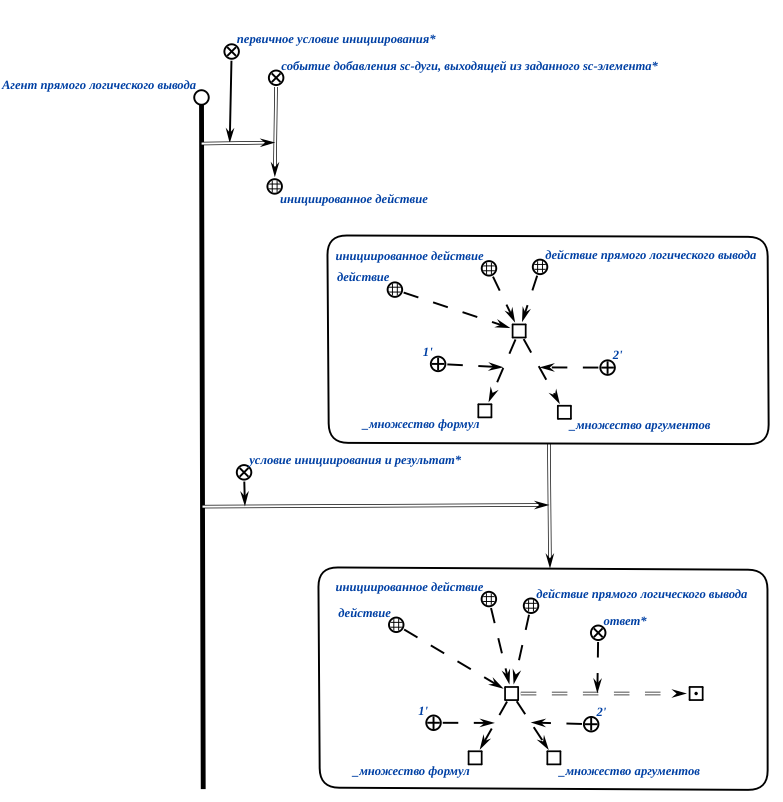
\includegraphics[scale=0.8]{author/part3/figures/direct_inference_agent.png}
	\label{fig:direct_inference_agent}
\end{figure}

Задачей \textit{Абстрактного sc-агента обратного логического вывода} является проверка гипотез. Некоторые гипотезы могут быть опровергнуты, однако извлекая причины того, почему гипотеза опровергнута, можно изменить посылку гипотезы так, чтобы создать новую гипотезу, которая впоследствии может стать полезной теоремой. Данный sc-агент активируется при появлении в sc-памяти инициированного действия, принадлежащего классу \textit{действие обратного логического вывода}. После проверки \textit{sc-агентом} условия инициирования выполняется процесс \textit{обратного логического вывода}, который схож с процессом \textit{прямого логического вывода} за исключением того, что поиск правил основывается не на посылках формул, а на их следствиях (см. \scncite{Gavrilova2001}). Ответом данного агента будет также дерево вывода, которое показывает, с использованием каких правил можно доказать или опровергнуть выдвинутую гипотезу.

\begin{SCn}
	\scnheader{Абстрактный sc-агент эквивалентных преобразований логической формулы}
	\begin{scnrelfromset}{декомпозиция абстрактного sc-агента}
		\scnitem{Абстрактный sc-агент преобразования формулы в конъюнктивную нормальную форму}
		\scnitem{Абстрактный sc-агент преобразования формулы в дизъюнктивную нормальную форму}
		\scnitem{Абстрактный sc-агент применения законов Де Моргана}
		\scnitem{Абстрактный sc-агент эквивалентных преобразований логической формулы по определению}
		\scnitem{Абстрактный sc-агент применения свойств отрицания логических формул}
		\scnitem{Абстрактный sc-агент применения закона идемпотентности логических формул}
		\scnitem{Абстрактный sc-агент применения закона коммутативности логических формул}
		\scnitem{Абстрактный sc-агент применения закона ассоциативности логических формул}
		\scnitem{Абстрактный sc-агент применения закона поглощения логических формул}
		\scnitem{Абстрактный sc-агент применения закона противоречия логических формул}
		\scnitem{Абстрактный sc-агент применения закона двойного отрицания логических формул}
		\scnitem{Абстрактный sc-агент применения закона расщепления логических формул}
	\end{scnrelfromset}
\end{SCn}

Любая формула семантически эквивалентна некоторой формуле в конъюнктивной нормальной форме, в связи с этим иногда удобно применять правило резолюции. Используя законы Де Моргана можно также получить формулы, пригодные для использования правила резолюции.
С помощью правила резолюции можно эффективно доказывать формулы \textit{Языка логики высказываний}.

Однако ничего принципиально нового правильно резолюции не привносит, поскольку формула $A \Rightarrow B$  равносильно $\neg A \lor B$ и из выводимости A и $A \rightarrow B$ следует выводимость B.

\begin{figure}[H]
	\caption{SCg-текст. Формализация конъюнктивной нормальной формы для импликации}
	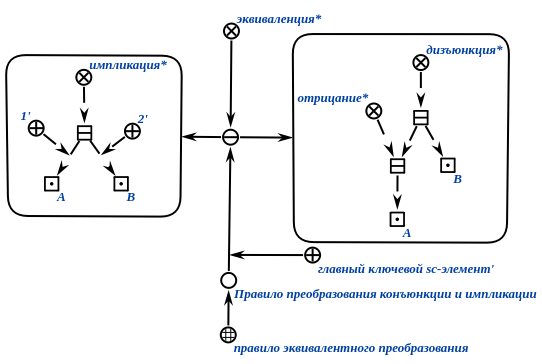
\includegraphics[scale=0.6]{author/part3/figures/conjunction_implication_rule.png}
	\label{fig:conjunction_implication_rule}
\end{figure}

Если в любых двух дизъюнктах $C_1$ и $C_2$ имеется пара формул $A$ и $\neg A$, то можно сформировать новый дизъюнкт из оставшихся частей изначальных дизъюнктов.

\begin{figure}[H]
	\caption{SCg-текст. Формализация правила резолюции}
	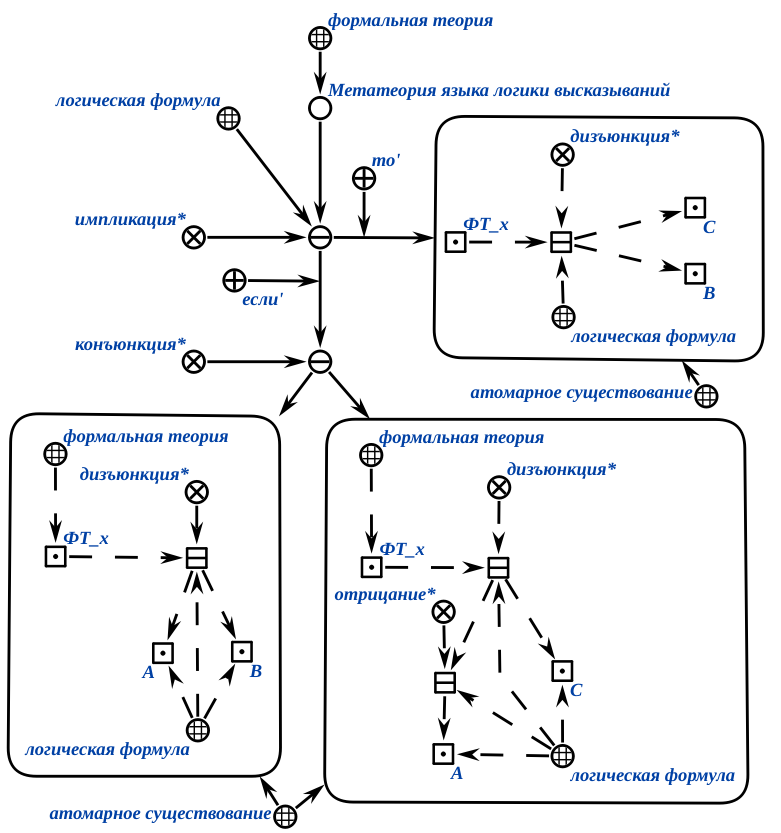
\includegraphics[scale=0.6]{author/part3/figures/resolution.png}
	\label{fig:resolution}
\end{figure}

Приведем пример вывода формулы из множества посылок, используя правило резолюции.
Если команда A выигрывает в футбол, то город A' торжествует, а если выигрывает команда B, то торжествовать будет город B'. Выиграть может или только город A', или только город B'. Однако, если выигрывает команда A, то город B' не торжествует, а если выигрывает команда B, то не торжествует город A'. Следовательно, город B' торжествует тогда и только тогда, когда не будет торжествовать город A'. Цель логического вывода - удостовериться, что город B' торжествует тогда и только тогда, когда не будет торжествовать город A'. Доказать вывода формулы равносильно доказательству противоречивости вывода отрицания этой формулы. При использовании правила резолюции это особенно удобно использовать.
Формализация логических формул, соответствующих примеру приведена на рисунке \textit{\nameref{fig:resolution_formulas_example}}. Каждая неатомарная формула на рисунке принадлежит некоторой формальной теории, то есть считается истинной.

\begin{figure}[H]
	\caption{SCg-текст. Формализация правил для применения правила резолюции}
	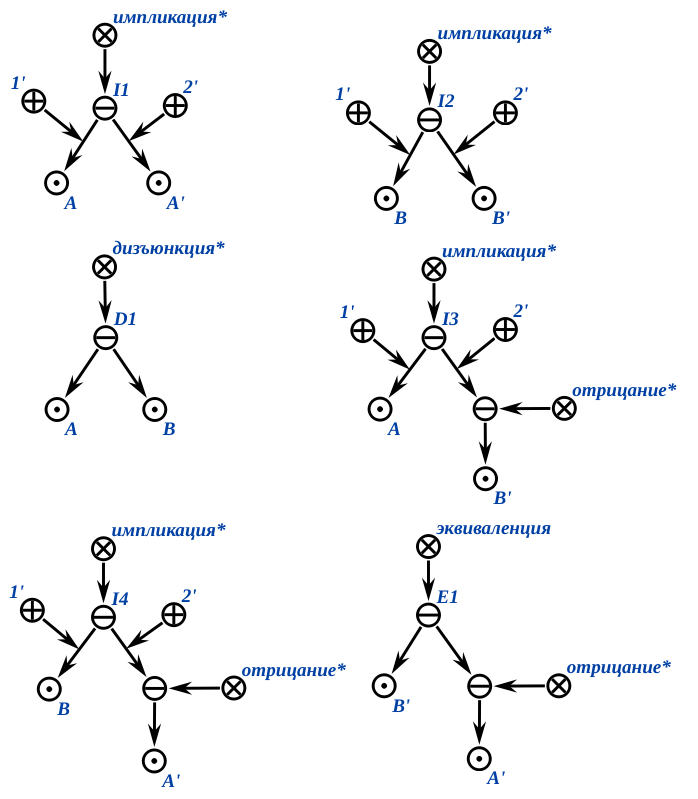
\includegraphics[scale=0.8]{author/part3/figures/resolution_formulas_example.png}
	\label{fig:resolution_formulas_example}
\end{figure}

Структура A представляет собой атомарную логическую формулу, которая обозначает победу команды A, структура A' представляет формулу, обозначающую торжество города A'. Соответственно, то же самое для структур B и B'.
Выразим логические формулы в булевом базисе. Прежде всего необходимо привести импликацию в конъюнктивную нормальную форму по формуле \textit{\nameref{fig:conjunction_implication_rule}} и эквиваленцию по определению. Затем применим отрицание к формуле, которую необходимо вывести (эвиваленция). В результате получим следующие формулы (рисунок \textit{\nameref{fig:resolution_prepared_formulas}}):

\begin{figure}[H]
	\caption{SCg-текст. Формализация правил для применения правила резолюции после преобразования в конъюнктивную нормальную форму}
	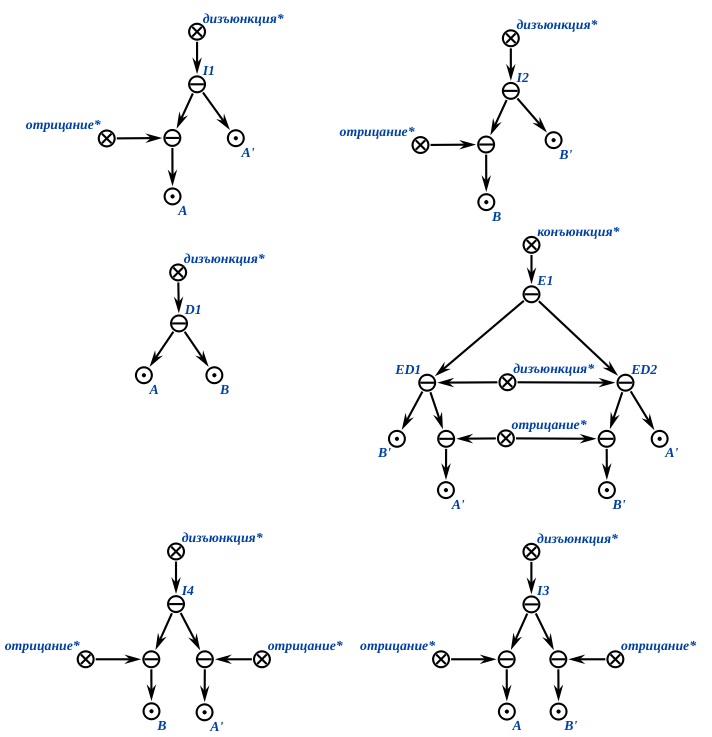
\includegraphics[scale=0.8]{author/part3/figures/resolution_prepared_formulas_example.png}
	\label{fig:resolution_prepared_formulas}
\end{figure}

Далее применяя правило резолюции для преобразованных формул получаем пустой дизъюнкт, что говорит о противоречивости множества формул и доказывает формулу эквиваленции о том, что город B' торжествует тогда и только тогда, когда не будет торжествовать город A'.

\begin{figure}[H]
	\caption{SCg-текст. Применение принципа резолюции}
	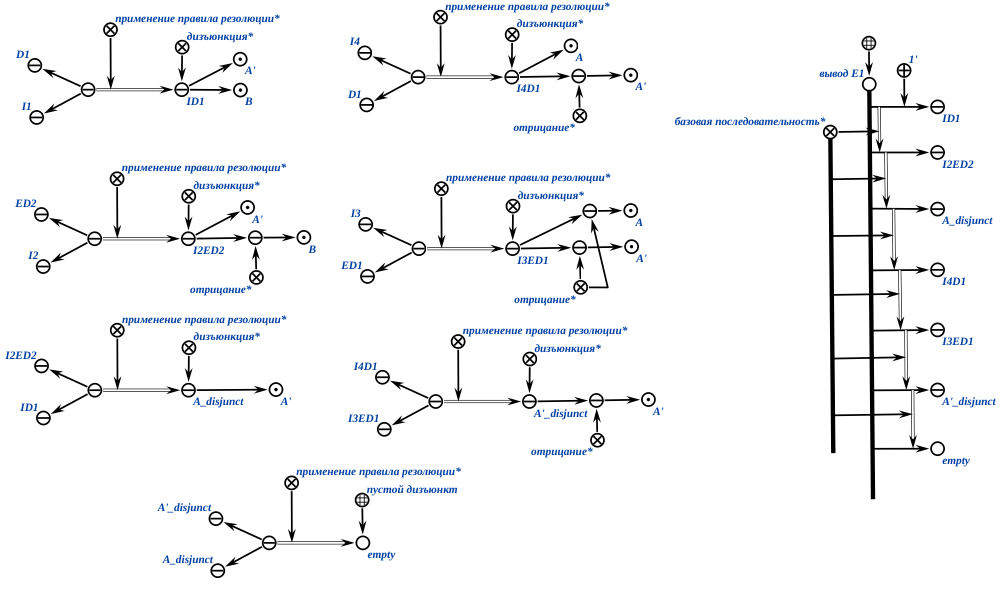
\includegraphics[scale=0.7]{author/part3/figures/resolution_inference.png}
	\label{fig:resolution_inference}
\end{figure}

Таким образом, можно использовать различные правила вывода, различные агенты логического вывода в различных видах логик в зависимости от специфики предметной области, в которой решается задача. Каждая модель является совместимой в рамках общей формальной модели решателей задач ostis-систем.

\section{Языки продукционного программирования, используемые ostis-системами}
\label{sec_logic_productions}

\begin{SCn}
	\begin{scnrelfromlist}{подраздел}
		\scnitem{\ref{subsec_prod_syntax}~\nameref{subsec_prod_syntax}}
		\scnitem{\ref{subsec_prod_sem}~\nameref{subsec_prod_sem}}
	\end{scnrelfromlist}
\end{SCn}

Продукции наряду с фреймами являются наиболее популярными средствами представления знаний в интеллектуальных компьютерных системах. Продукции, с одной стороны, близки к  логическим моделям, что позволяет организовывать на них эффективные процедуры вывода, а с другой стороны, более наглядно отражают знания, чем классические логические модели. В них отсутствуют жесткие ограничения, характерные для логических исчислений, что дает возможность изменять  
интерпретацию элементов продукции.

Так как в основе \textit{Технологии OSTIS} лежит \textit{многоагентный подход}, который позволяет легко интерпретировать любую информацию, то можно сделать вывод, что продукционный подход легко интегрируется в \textit{решатели задач} \textit{ostis-систем} в виде \textit{sc-агентов}.  Интеграция \textit{Технологии OSTIS} и продукционного подхода позволяет объединить статические и динамические знания в рамках единого формализма, а также получить их графическое представление.

\subsection{Синтаксис языков продукционного программирования, используемых ostis-системами}
\label{subsec_prod_syntax}

В общем виде под продукцией понимается выражение следующего вида:

($i$); $Q$; $P$; $A$ $\Rightarrow$ $B$; $N$.

Здесь $i$ --- имя продукции, с помощью которого данная продукция выделяется из всего множества продукций. В качестве имени может выступать некоторая лексема, отражающая суть данной продукции (например, "покупка книги"{} или "набор кода замка"{}), или порядковый номер продукции в их множестве, хранящемся в памяти системы. 

Элемент $Q$ характеризует сферу применения продукции или же контекст. 

Основным элементом продукции является ее ядро: $A$ $\Rightarrow$ $B$. Интерпретация ядра продукции может быть различной и зависит от того, что стоит слева и справа от знака секвенции $\Rightarrow$. Обычное прочтение ядра продукции выглядит так: ЕСЛИ $A$, ТО $B$, более сложные конструкции ядра допускают в правой части альтернативный выбор, например, ЕСЛИ $A$, ТО $B_1$ ИНАЧЕ $B_2$. Секвенция может истолковываться в обычном логическом смысле как знак логического следования $B$ из истинного $A$ (если $A$ не является истинным выражением, то о $B$ ничего сказать нельзя). Возможны и другие интерпретации ядра продукции, например $A$ описывает некоторое условие, необходимое для того, чтобы можно было совершить действие $B$.

Элемент $P$ есть условие применимости ядра продукции. Обычно $P$ представляет собой логическое выражение (как правило, предикат). Когда $P$ принимает значение «истина», ядро продукции активизируется. Если $P$ ложно, то ядро продукции не может быть использовано. Например, если в продукции «НАЛИЧИЕ ДЕНЕГ; ЕСЛИ ХОЧЕШЬ КУПИТЬ ВЕЩЬ X, ТО ЗАПЛАТИ В КАССУ ЕЕ СТОИМОСТЬ И ОТДАЙ ЧЕК ПРОДАВЦУ» условие применимости ядра продукции ложно, то есть денег нет, то применить ядро продукции невозможно.

Элемент $N$ описывает постусловия продукции. Они актуализируются только в том случае, если ядро продукции реализовалось. Постусловия продукции описывают действия и процедуры, которые необходимо выполнить после реализации В. Например, после покупки некоторой вещи в магазине необходимо в описи товаров, имеющихся в этом магазине, уменьшить количество вещей такого типа на единицу. Выполнение $N$ может происходить не сразу после реализации ядра продукции (см. \scncite{AIHandbookMM}).

Если в памяти системы хранится некоторый набор продукций, то они образуют систему продукций. В системе продукций должны быть заданы специальные процедуры управления продукциями, с помощью которых происходит актуализация продукций и выбор для выполнения той или иной продукции из числа актуализированных.

Продукционный язык программирования в общем случае может содержать структурные единицы различного характера. Это могут быть определения глобальных переменных, операторы управления макрогенерацией, вставки текстов на алгоритмических языках программирования и целый ряд других элементов. Однако основной единицей продукционного языка программирования, определяющей его лицо и его возможности, является продукция.

В ряде интеллектуальных систем используются комбинации сетевых и продукционных моделей представления знаний. В таких моделях декларативные знания описываются в сетевом компоненте модели, а процедурные знания --- в продукционном. В этом случае говорят о работе продукционной системы над семантической сетью. Процедурные знания позволяют системе узнать, как можно использовать те или иные декларативные знания, в частности, знания о закономерностях той части действительности, в которой "живет"{} интеллектуальная система, для получения нужных системе результатов или тех результатов, которые ожидает от нее пользователь.



\subsection{Денотационная семантика языков продукционного программирования, используемых ostis-системами}
\label{subsec_prod_sem}

Одним из наиболее известных языков этого класса является \textbf{\textit{OPS5}}. \textit{OPS5} можно рассматривать как полноценный язык программирования для продукционного программирования.
База данных в языке называется рабочей памятью (working memory) и состоит из нескольких сотен объектов, каждый из ко­торых имеет свой набор атрибутов. Объект вместе с парами <атрибут -- значение> называется элементом рабочей памяти (см. \scncite{Brownston1985}). 

Основная задача, которую поставили перед собой разработчики языка \textit{OPS5}, добиться максимально высокой эффективности выполнения про­дукционной программы. Интерпретатор системы порождает конфликт­ное множество, каждый элемент которого представляет собой пару <имя продукции, список элементов рабочей памяти, которые являются означи­ваниями для образцов продукции>. Каждая продукция в \textit{OPS5} состоит из символа Р, имени продукции, левой части, символа --> и правой части.

В \textit{OPS5} вы­делены три типа действий:
\begin{textitemize}
	\item{MAKE --- создает новый элемент рабочей памяти;}
	\item{MODIFY --- изменяет один или несколько значений атрибутов у существующего элемента рабочей памяти;}
	\item{REMOVE --- удаляет элемент рабочей памяти.}
\end{textitemize}

\begin{figure}[H]
	\caption{Рисунок. Пример правила продукции на OPS5}
	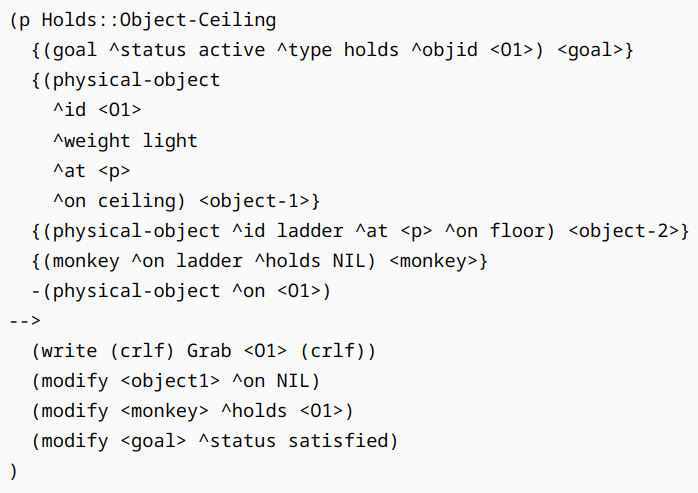
\includegraphics[scale=0.4]{author/part3/figures/ops5_production_rule_example.png}
	\label{fig:ops5_production_rule_example}
\end{figure}
В этом примере данные в рабочей памяти структурированы и переменные появляются в угловых скобках. Название структуры данных, такое как "goal"{} (цель) и "physical-object"{} (физический объект), является первым буквальным в условиях; поля структуры начинаются с "\textasciicircum"{}. На негативное состояние  указывает "{}--"{}.

Продукционные правила в \textit{OPS5} применяются ко всем продукциям структур данных, которые соответствуют условиям и соответствуют привязкам переменных. В этом примере, если несколько объектов подвешены к потолку, каждый с другой лестницей рядом, поддерживающей обезьяну с пустыми руками, конфликтный набор будет содержать столько же продукций правил продукции, полученных из одной и той же продукции "Holds::Object-Ceiling"{}. На этапе разрешения конфликта позже будет выбрано, какие продукции запускать.

Связывание переменных, возникающее в результате сопоставления с шаблоном в левой части, используется в правой части для ссылки на данные, подлежащие модификации. Рабочая память содержит явные данные структуры управления в виде экземпляров «целевой» структуры данных. В этом примере, когда обезьяна держит подвешенный объект, статус цели устанавливается на «удовлетворено», и то же производственное правило больше не может применяться, поскольку его первое условие не выполняется.

\textbf{\textit{CLIPS}} использует продукционную модель представления знаний и поэтому содержит три основных элемента:
\begin{textitemize}
	\item{базу фактов (fact base),}
	\item{базу правил (rule base),}
	\item{механизм логического вывода.}
\end{textitemize}
База фактов представляет исходное описание задачи. База правил содержит операторы, которые преобразуют состояния проблемы, приводя его к решению --- целевому состоянию (см. \scncite{CLIPS}).

Механизм логического вывода \textit{CLIPS} сопоставляет факты из базы фактов и правила из базы правил и выясняет, какие из правил можно активизировать. Это выполняется циклически, причем каждый цикл (так называемый продукционный цикл или цикл распознавания действия) состоит из трех основных фаз:
\begin{textitemize}
	\item{сопоставление фактов и правил;}
	\item{выбор правила, подлежащего активизации;}
	\item{выполнение действий, предписанных активным («зажженным») правилом.}
\end{textitemize}

Факты --- это одна из основных форм представления информации в системе \textit{CLIPS}. Каждый факт представляет фрагмент информации, который был помещен в текущий список фактов, называемый fact-list. Факт представляет собой основную единицу данных, используемую правилами.

Если при добавлении нового факта к списку обнаруживается, что он полностью совпадает с одним из уже включенных в список фактов, то эта операция игнорируется.

Факт может описываться индексом или адресом. Всякий раз, когда факт добавляется (изменяется), ему присваивается уникальный целочисленный индекс. Факт также может задаваться при помощи адреса.

Идентификатор факта --- это короткая запись для отображения факта на экране. Она состоит из символа f и записанного через тире индекса факта. Существует два формата представления фактов: позиционный и непозиционный. Позиционные факты состоят из выражения символьного типа, за которым следует последовательность (возможно, пустая) из полей, разделенных пробелами. Вся запись заключается в скобки. Обычно первое поле определяет "отношение"{}, которое применяется к оставшимся полям.


\textbf{\textit{Алгоритм Rete}} содержит обобщение логики функционала, ответственного за связь данных (фактов) и алгоритма (продукций) в системах сопоставления с образцом (вид систем: системы основанные на правилах). Продукция состоит из одного или нескольких условий и набора действий, выполняемых если актуальный набор фактов соответствует одному из условий. Условия накладываются на атрибуты фактов, включая их типы и идентификаторы. \textit{Алгоритм Rete} имеет следующие характеристики:
\begin{textitemize}
	\item{Уменьшает или исключает избыточность условий за счет объединения узлов.}
	\item{Сохраняет частичные соответствия между фактами при слиянии разных типов фактов. Это позволяет избежать полного вычисления всех фактов при любом изменении в рабочей памяти продукционной системы. Система работает только с самими изменениям.}
	\item{Позволяет эффективно высвобождать память при удалении фактов.}
\end{textitemize}

\textit{Алгоритм Rete} широко используется для реализации сопоставления с образцом в системах с циклом сопоставление-решение-действие для генерации и логического вывода (см. \scncite{Forgy1982}).

\textit{Rete II} улучшен по двум параметрам: повышена общая производительность сети включая хешированную память для больших массивов данных, добавлен алгоритм обратного вывода, работающий на той же сети. Скорость обратного вывода по сравнению с \textit{Rete I} повышена значительно.

\textit{Rete-NT} --- новое поколение \textit{алгоритма Rete}. Алгоритм был признан более быстрым, чем оригинальный \textit{алгоритм Rete} и в 10 раз более быстрым, чем его предшественник \textit{Rete II}. 

\textbf{\textit{Миварный подход}} объединяет и другие научные области компьютерных наук, информатики и дискретной математики, включая: базы данных, экспертные системы, системы логического вывода на основе развития продукций, теорию графов, матрицы, параллельное выполнение программ на кластерах, проектирование новых архитектур компьютеров, массовое суммирование чисел, техническую защиту информации и информационную безопасность, гносеологию (частично и в плане создания новой наиболее мощной модели данных на основе "тройки"{} "вещь-свойство-отношение"{}), сервисно-ориентированные архитектуры, компьютерные сети, информационные инфраструктуры, теоретическую робототехнику, многоагентные системы и некоторые другие (см. \scncite{Vladimirov2010}). \textit{Миварный подход} объединяет две основные технологии накопления данных и обработки информации:

\begin{textitemize}
	\item{миварное информационное пространство: накопление данных на основе эволюционной самоорганизующейся миварной модели данных с изменяющейся структурой в теории баз данных,}
	\item{миварные сети: обработка информации на основе развития продукционного подхода к логическому выводу с учетом включения возможности автоматического конструирования алгоритмов для "решателей задач"{} и традиционной вычислительной обработки, а также с использованием идей отношений, правил и процедур, которые теперь принято относить к сервисно-ориентированным архитектурам и многоагентным системам.}
\end{textitemize}


Суть \textit{миварного подхода} в объединении баз данных и систем логико-вычислительной обработки в единые эволюционно развивающиеся системы, позволяющие собрать воедино все различные научные разработки на основе сервисно-ориентированных архитектур и технологий интеллектуальных агентов --- многоагентных систем. 

Миварные сети основаны на продукционном подходе "если, то…"{} с переходом к более сложной структуре правил с предусловиями, условиями, ограничениями, действиями и последействиями. Это позволяет записывать все причинно-следственные отношения, включая и все возможные формы предикатов и подобных логических выражений. Мы не отрицаем значение предикатов и поиска истинных выражений, а только создаем возможность и для их реализации, и для реализации всех возможных других представлений правил в виде: сервисов, процедур, продукций, подпрограмм и так далее. Такой подход позволяет работать одновременно с разными описаниями предметных областей, прибавляя к предикатам и продукции, и нейросети, и генетические алгоритмы, и традиционные вычислительные процедуры, и все другие в виде универсальных миварных отношений, которые представляются и хранятся перед обработкой в нашем миварном пространстве. 

%%%%%%%%%%%%%%%%%%%%%%%%% referenc.tex %%%%%%%%%%%%%%%%%%%%%%%%%%%%%%
% sample references
% %
% Use this file as a template for your own input.
%
%%%%%%%%%%%%%%%%%%%%%%%% Springer-Verlag %%%%%%%%%%%%%%%%%%%%%%%%%%
%
% BibTeX users please use
% \bibliographystyle{}
% \bibliography{}
%
\biblstarthook{In view of the parallel print and (chapter-wise) online publication of your book at \url{www.springerlink.com} it has been decided that -- as a genreral rule --  references should be sorted chapter-wise and placed at the end of the individual chapters. However, upon agreement with your contact at Springer you may list your references in a single seperate chapter at the end of your book. Deactivate the class option \texttt{sectrefs} and the \texttt{thebibliography} environment will be put out as a chapter of its own.\\\indent
References may be \textit{cited} in the text either by number (preferred) or by author/year.\footnote{Make sure that all references from the list are cited in the text. Those not cited should be moved to a separate \textit{Further Reading} section or chapter.} If the citatiion in the text is numbered, the reference list should be arranged in ascending order. If the citation in the text is author/year, the reference list should be \textit{sorted} alphabetically and if there are several works by the same author, the following order should be used:
\begin{enumerate}
\item all works by the author alone, ordered chronologically by year of publication
\item all works by the author with a coauthor, ordered alphabetically by coauthor
\item all works by the author with several coauthors, ordered chronologically by year of publication.
\end{enumerate}
The \textit{styling} of references\footnote{Always use the standard abbreviation of a journal's name according to the ISSN \textit{List of Title Word Abbreviations}, see \url{http://www.issn.org/en/node/344}} depends on the subject of your book:
\begin{itemize}
\item The \textit{two} recommended styles for references in books on \textit{mathematical, physical, statistical and computer sciences} are depicted in ~\cite{science-contrib, science-online, science-mono, science-journal, science-DOI} and ~\cite{phys-online, phys-mono, phys-journal, phys-DOI, phys-contrib}.
\item Examples of the most commonly used reference style in books on \textit{Psychology, Social Sciences} are~\cite{psysoc-mono, psysoc-online,psysoc-journal, psysoc-contrib, psysoc-DOI}.
\item Examples for references in books on \textit{Humanities, Linguistics, Philosophy} are~\cite{humlinphil-journal, humlinphil-contrib, humlinphil-mono, humlinphil-online, humlinphil-DOI}.
\item Examples of the basic Springer style used in publications on a wide range of subjects such as \textit{Computer Science, Economics, Engineering, Geosciences, Life Sciences, Medicine, Biomedicine} are ~\cite{basic-contrib, basic-online, basic-journal, basic-DOI, basic-mono}. 
\end{itemize}
}

\begin{thebibliography}{99.}%
% and use \bibitem to create references.
%
% Use the following syntax and markup for your references if 
% the subject of your book is from the field 
% "Mathematics, Physics, Statistics, Computer Science"
%
% Contribution 
\bibitem{science-contrib} Broy, M.: Software engineering --- from auxiliary to key technologies. In: Broy, M., Dener, E. (eds.) Software Pioneers, pp. 10-13. Springer, Heidelberg (2002)
%
% Online Document
\bibitem{science-online} Dod, J.: Effective substances. In: The Dictionary of Substances and Their Effects. Royal Society of Chemistry (1999) Available via DIALOG. \\
\url{http://www.rsc.org/dose/title of subordinate document. Cited 15 Jan 1999}
%
% Monograph
\bibitem{science-mono} Geddes, K.O., Czapor, S.R., Labahn, G.: Algorithms for Computer Algebra. Kluwer, Boston (1992) 
%
% Journal article
\bibitem{science-journal} Hamburger, C.: Quasimonotonicity, regularity and duality for nonlinear systems of partial differential equations. Ann. Mat. Pura. Appl. \textbf{169}, 321--354 (1995)
%
% Journal article by DOI
\bibitem{science-DOI} Slifka, M.K., Whitton, J.L.: Clinical implications of dysregulated cytokine production. J. Mol. Med. (2000) doi: 10.1007/s001090000086 
%
\bigskip

% Use the following (APS) syntax and markup for your references if 
% the subject of your book is from the field 
% "Mathematics, Physics, Statistics, Computer Science"
%
% Online Document
\bibitem{phys-online} J. Dod, in \textit{The Dictionary of Substances and Their Effects}, Royal Society of Chemistry. (Available via DIALOG, 1999), 
\url{http://www.rsc.org/dose/title of subordinate document. Cited 15 Jan 1999}
%
% Monograph
\bibitem{phys-mono} H. Ibach, H. L\"uth, \textit{Solid-State Physics}, 2nd edn. (Springer, New York, 1996), pp. 45-56 
%
% Journal article
\bibitem{phys-journal} S. Preuss, A. Demchuk Jr., M. Stuke, Appl. Phys. A \textbf{61}
%
% Journal article by DOI
\bibitem{phys-DOI} M.K. Slifka, J.L. Whitton, J. Mol. Med., doi: 10.1007/s001090000086
%
% Contribution 
\bibitem{phys-contrib} S.E. Smith, in \textit{Neuromuscular Junction}, ed. by E. Zaimis. Handbook of Experimental Pharmacology, vol 42 (Springer, Heidelberg, 1976), p. 593
%
\bigskip
%
% Use the following syntax and markup for your references if 
% the subject of your book is from the field 
% "Psychology, Social Sciences"
%
%
% Monograph
\bibitem{psysoc-mono} Calfee, R.~C., \& Valencia, R.~R. (1991). \textit{APA guide to preparing manuscripts for journal publication.} Washington, DC: American Psychological Association.
%
% Online Document
\bibitem{psysoc-online} Dod, J. (1999). Effective substances. In: The dictionary of substances and their effects. Royal Society of Chemistry. Available via DIALOG. \\
\url{http://www.rsc.org/dose/Effective substances.} Cited 15 Jan 1999.
%
% Journal article
\bibitem{psysoc-journal} Harris, M., Karper, E., Stacks, G., Hoffman, D., DeNiro, R., Cruz, P., et al. (2001). Writing labs and the Hollywood connection. \textit{J Film} Writing, 44(3), 213--245.
%
% Contribution 
\bibitem{psysoc-contrib} O'Neil, J.~M., \& Egan, J. (1992). Men's and women's gender role journeys: Metaphor for healing, transition, and transformation. In B.~R. Wainrig (Ed.), \textit{Gender issues across the life cycle} (pp. 107--123). New York: Springer.
%
% Journal article by DOI
\bibitem{psysoc-DOI}Kreger, M., Brindis, C.D., Manuel, D.M., Sassoubre, L. (2007). Lessons learned in systems change initiatives: benchmarks and indicators. \textit{American Journal of Community Psychology}, doi: 10.1007/s10464-007-9108-14.
%
%
% Use the following syntax and markup for your references if 
% the subject of your book is from the field 
% "Humanities, Linguistics, Philosophy"
%
\bigskip
%
% Journal article
\bibitem{humlinphil-journal} Alber John, Daniel C. O'Connell, and Sabine Kowal. 2002. Personal perspective in TV interviews. \textit{Pragmatics} 12:257--271
%
% Contribution 
\bibitem{humlinphil-contrib} Cameron, Deborah. 1997. Theoretical debates in feminist linguistics: Questions of sex and gender. In \textit{Gender and discourse}, ed. Ruth Wodak, 99--119. London: Sage Publications.
%
% Monograph
\bibitem{humlinphil-mono} Cameron, Deborah. 1985. \textit{Feminism and linguistic theory.} New York: St. Martin's Press.
%
% Online Document
\bibitem{humlinphil-online} Dod, Jake. 1999. Effective substances. In: The dictionary of substances and their effects. Royal Society of Chemistry. Available via DIALOG. \\
http://www.rsc.org/dose/title of subordinate document. Cited 15 Jan 1999
%
% Journal article by DOI
\bibitem{humlinphil-DOI} Suleiman, Camelia, Daniel C. O'Connell, and Sabine Kowal. 2002. `If you and I, if we, in this later day, lose that sacred fire...': Perspective in political interviews. \textit{Journal of Psycholinguistic Research}. doi: 10.1023/A:1015592129296.
%
%
%
\bigskip
%
%
% Use the following syntax and markup for your references if 
% the subject of your book is from the field 
% "Computer Science, Economics, Engineering, Geosciences, Life Sciences"
%
%
% Contribution 
\bibitem{basic-contrib} Brown B, Aaron M (2001) The politics of nature. In: Smith J (ed) The rise of modern genomics, 3rd edn. Wiley, New York 
%
% Online Document
\bibitem{basic-online} Dod J (1999) Effective Substances. In: The dictionary of substances and their effects. Royal Society of Chemistry. Available via DIALOG. \\
\url{http://www.rsc.org/dose/title of subordinate document. Cited 15 Jan 1999}
%
% Journal article by DOI
\bibitem{basic-DOI} Slifka MK, Whitton JL (2000) Clinical implications of dysregulated cytokine production. J Mol Med, doi: 10.1007/s001090000086
%
% Journal article
\bibitem{basic-journal} Smith J, Jones M Jr, Houghton L et al (1999) Future of health insurance. N Engl J Med 965:325--329
%
% Monograph
\bibitem{basic-mono} South J, Blass B (2001) The future of modern genomics. Blackwell, London 
%
\end{thebibliography}
